\hypertarget{abstract}{%
\section{Abstract}\label{abstract}}

\(x = 3\)

The necessity of intervention in inferring cause has long been
understood in neuroscience. Recent work has highlighted the limitations
of passive observation and single-site lesion studies in accurately
recovering causal circuit structure. The advent of optogenetics has
facilitated increasingly precise forms of intervention including
closed-loop control which may help eliminate confounding influences.
However, it is not yet clear how best to apply closed-loop control to
leverage this increased inferential power. In this paper, we use tools
from causal inference, control theory, and neuroscience to show when and
how closed-loop interventions can more effectively reveal causal
relationships.
\texttt{We\ also\ examine\ the\ performance\ of\ standard\ network\ inference\ procedures\ in\ simulated\ spiking\ networks\ under\ passive,\ open-loop\ and\ closed-loop\ conditions.}
We demonstrate a unique capacity of feedback control to distinguish
competing circuit hypotheses by disrupting connections which would
otherwise result in equivalent patterns of correlation\footnote{may end
  up discussing quantitative advantages such as bidirectional variance
  (and correlation) control. If that's a strong focus in the results,
  should be talked about more in the abstract also}. Our results build
toward a practical framework to improve design of neuroscience
experiments to answer causal questions about neural circuits.

\hypertarget{introduction}{%
\section{Introduction}\label{introduction}}

\hypertarget{estimating-causal-interactions-in-the-brain}{%
\subsection{Estimating causal interactions in the
brain}\label{estimating-causal-interactions-in-the-brain}}

Many hypotheses about neural circuits are phrased in terms of causal
relationships: ``will changes in activity to this region of the brain
produce corresponding changes in another region?'' Understanding these
causal relationships is critical to both scientific understanding and to
developing effective therapeutic interventions, which require knowledge
of how potential therapies will impact brain activity and patient
outcomes.

A range of mathematical and practical challenges make it difficult to
determine these causal relationships. In studies that rely only
observational data, it is often impossible to determine whether observed
patterns of activity are caused by known and controlled inputs, or
whether they are instead spurious connections generated by recurrent
activity, indirect relationships, or unobserved ``confounders.'' It is
generally understood that moving from experiments involving passive
observation to more complex levels of intervention allows experimenters
to better tackle challenges to circuit identification. However, while
chemical and surgical lesion experiments have historically been employed
to remove the influence of possible confounds, they are likely to
dramatically disrupt circuits from their typical functions, making
conclusions about underlying causal structure drawn from these
experiments unlikely to hold in naturalistic settings .
\emph{Closed-loop} interventions {[}\ldots{]} short description of
closed-loop in neuro, maybe drawing from text in this

Despite the promise of these closed-loop strategies for identifying
causal relations in neural circuits, however, it is not yet fully
understood \emph{when} more complex intervention strategies can provide
additional inferential power, or \emph{how} these experiments should be
optimally designed. In this paper we demonstrate when and how
closed-loop interventions can reveal the causal structure governing
neural circuits. Drawing from ideas in causal inference , we describe
the classes of models that can be distinguished by a given set of
input-output experiments, and what experiments are necessary to uniquely
determine specific causal relationships.

We first propose a mathematical framework that describes how open- and
closed-loop interventions impact observable qualities of neural
circuits. Using this framework, experimentalists propose a set of
candidate hypotheses describing the potential causal structure of the
circuit under study, and then select a series of interventions that best
allows them to distinguish between these hypotheses. Using both simple
controlled models and in silico models of spiking networks, we explore
factors that govern the efficacy of these types of interventions. Guided
by the results of this exploration, we present a set of recommendations
that can guide the design of open- and closed-loop experiments to better
uncover the causal structure underlying neural circuits.

\textbf{Inferring causal interactions from time series.} A number of
strategies have been proposed to detect causal relationships between
observed variables. Wiener-Granger (or predictive) causality states that
a variable \(X\) ``Granger-causes'' \(Y\) if \(X\) contains information
relevant to \(Y\) that is not contained in \(Y\) itself or any other
variable . This concept has traditionally been operationalized with
vector autoregressive models ; the requirement that \emph{all}
potentially causative variables be considered makes these notions of
dependence susceptible to unobserved confounders .

Our work initially focuses on measures of directional interaction that
are based on lagged correlations . These metrics look at the correlation
of time series collected from pairs of nodes at various lags and detect
peaks at negative time lags. Such peaks could indicate the presence of a
direct causal relationship -- but they could also stem from indirect
causal links or hidden confounders . In these bivariate correlation
methods, it is thus necessary to consider patterns of correlation
between many pairs of nodes in order to differentiate between direct,
indirect, and confounding relationships . This distinguishes these
strategies from some multivariate methods that ``control'' for the
effects of potential confounders. While cross-correlation-based measures
are generally limited to detecting linear functional relationships
between nodes, their computational feasibility makes them a frequent
metric of choice in experimental neuroscience work .

Other techniques detect directional interaction stemming from more
general or complex relationships. Information-theoretic methods, which
use information-based measures to assess the reduction in entropy
knowledge of one variable provides about another, are closely related to
Granger causality . The \emph{transfer entropy}
\(T_{X \to Y}(t) = I(Y_t \colon X_{<t} \mid Y_{<t})\) extends this
notion to time series by measuring the amount of information present in
\(Y_t\) that is not contained in the past of either \(X\) or \(Y\)
(denoted \(X_{<t}\) and \(Y_{<t}\)) . Using transfer entropy as a
measure of causal interaction requires accounting for potential
confounding variables; the \emph{conditional transfer entropy}
\(T_{X \to Y \mid Z}(t) = I(Y_t \colon X_{<t} \mid Y_{<t}, Z_{<t})\)
conditions on the past of other variables to account for their potential
confounding influence . Conditional transfer entropy can thus be
interpreted as the amount of information present in \(Y\) that is not
contained in the past of \(X\), the past of \(Y\), or the past of other
variables \(Z\).

To quantify the strength of causal interactions, information-theoretic
and transfer-entropy-based methods typically require knowledge of the
ground truth causal relationships that exist or an ability to perturb
the system . In practice, these quantities are typically interpreted as
``information transfer,'' and a variety of estimation strategies and
methods to automatically select the conditioning set (i.e., the
variables and time lags that should be conditioned on) are used (e.g.,
). Multivariate conditional transfer entropy approaches using various
variable selection schemes can differentiate between direct
interactions, indirect interactions, and common causes, but their
results depend on choices such as the binning strategies used to
discretize continuous signals, the specific statistical tests used, and
the estimator used to compute transfer entropy . However, despite their
mathematical differences, previous work has found that
cross-correlation-based metrics and information-based metrics tend to
produce qualitatively similar results, with similar patterns of true and
false positives .

\hypertarget{interventions-in-neuroscience-causal-inference}{%
\subsection{Interventions in neuroscience \& causal
inference}\label{interventions-in-neuroscience-causal-inference}}

Data collected from experimental settings can provide more inferential
power than observational data alone. For example, consider an
experimentalist who is considering multiple causal hypotheses for two
nodes under study, \(x\) and \(y\): the hypothesis that \(x\) is driving
\(y\), the hypothesis that \(y\) is driving \(x\), or the hypothesis
that the two variables are being independently driven by a hidden
confounder. Observational data revealing that \(x\) and \(y\) produce
correlated time-series data is equally consistent with each of these
three causal hypotheses, providing the experimentalist with no
inferential power. Experimentally manipulating \(x\) and observing the
output of \(y\), however, allows the scientist to begin to establish
which causal interaction pattern is at work. Consistent with intuition
from neuroscience literature, a rich theoretical literature has
described the central role of interventions in inferring causal
structure from data .

FIG: %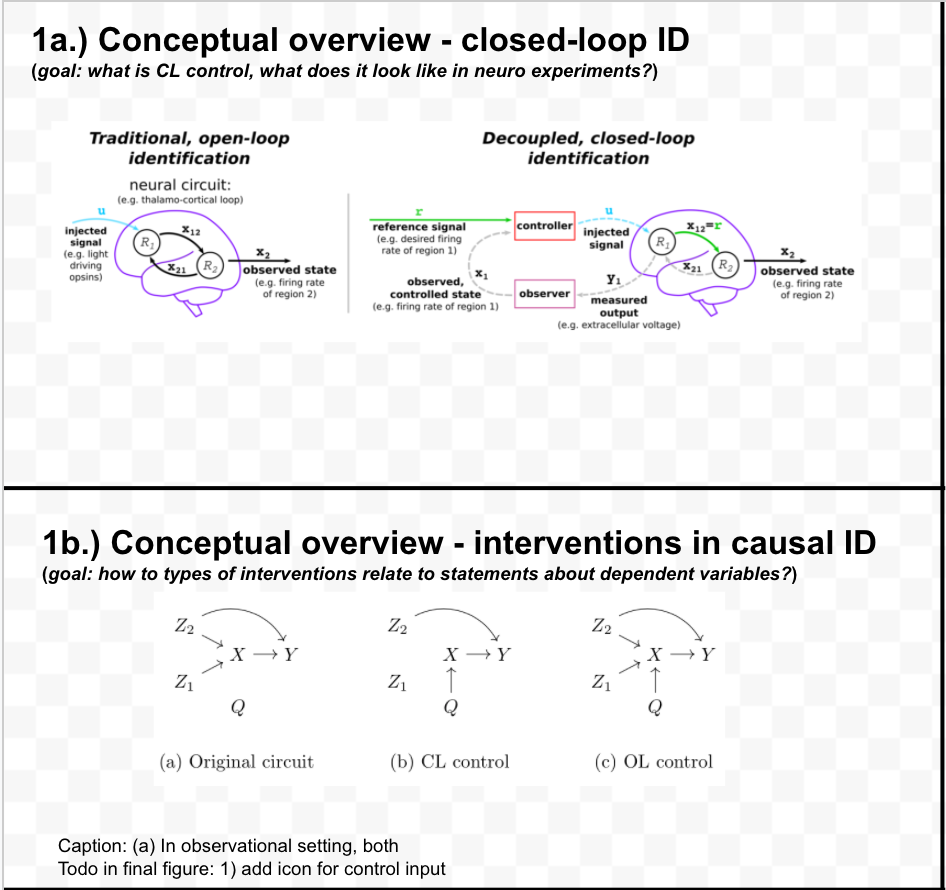
\includegraphics{figures/core_figure_sketches/figure1_sketch.png}
\textgreater{} \textbf{Figure INTRO:} Examples of the roles
interventions have played in neuroscience. (A) \emph{Passive
observation} does not involve stimulating the brain. In this example,
passive observational data is used to identify patients suffering from
absence seizures. (B) \emph{Open-loop stimulation} involves recording
activity in the brain after perturbing a region with a known input
signal. Using systematic \emph{open-loop stimulation experiments},
Penfield uncovered the spatial organization of how senses and movement
are mapped in the cortex . (C) \emph{Closed-loop control} uses feedback
control to precisely specify activity in certain brain regions
regardless of activity in other regions. Using closed-loop control, .

The inferential power of interventions is depends on \emph{where}
stimulation is applied: interventions on some portions of a system may
provide more information about the system's causal structure than
interventions in other areas. And interventions are also more valuable
when they more effectively set the state of the system: ``perfect''
closed-loop control, which completely severs a node's activity from its
inputs, are often more informative than ``soft'' interventions that only
partially control a part of the system .

In experimental neuroscience settings, experimenters are faced with
deciding between interventions that differ in both location and
effectiveness. For example, stimulation can often only be applied to
certain regions of the brain. And while experimenters may be able to
exactly manipulate activity in some parts of the brain using closed-loop
control, in other locations it may only be possible to apply weaker
forms of intervention that perturb a region but do not manipulate its
activity exactly to a desired state. In Section \texttt{X}, we compare
the effectiveness of open-loop, closed-loop, and partially-effective
closed-loop control.

Although algorithms designed to choose optimal interventions are often
designed for simple models with strong assumptions,\footnote{These
  assumptions are typically on properties such as the types of
  functional relationships that exist in circuits, the visibility and
  structure of confounding relationships, and noise statistics.} they
provide intuition that can aid practitioners seeking to design
real-world experiments that provide as much scientific insight as
possible.\footnote{if citations needed here, could start by looking for
  a good high-level reference in either or . (Both of these papers are
  pretty technical, so likely wouln't be great citations on their own.)}
Importantly, the informativeness of interventions is often independent
of the algorithm used to infer causal connections, meaning that certain
interventions can reveal portions of a circuit's causal structure that
would be impossible for \emph{any} algorithm to infer from only
observational data Matt to Adam: make sure this citation is in the right
We similarly expect the results we demonstrate in this paper to both
inform experimentalists and open avenues for further research.

\hypertarget{representations-reachability}{%
\subsection{Representations \&
reachability}\label{representations-reachability}}

import ``/section\_content/background\_representation\_reach.md''

FIG: %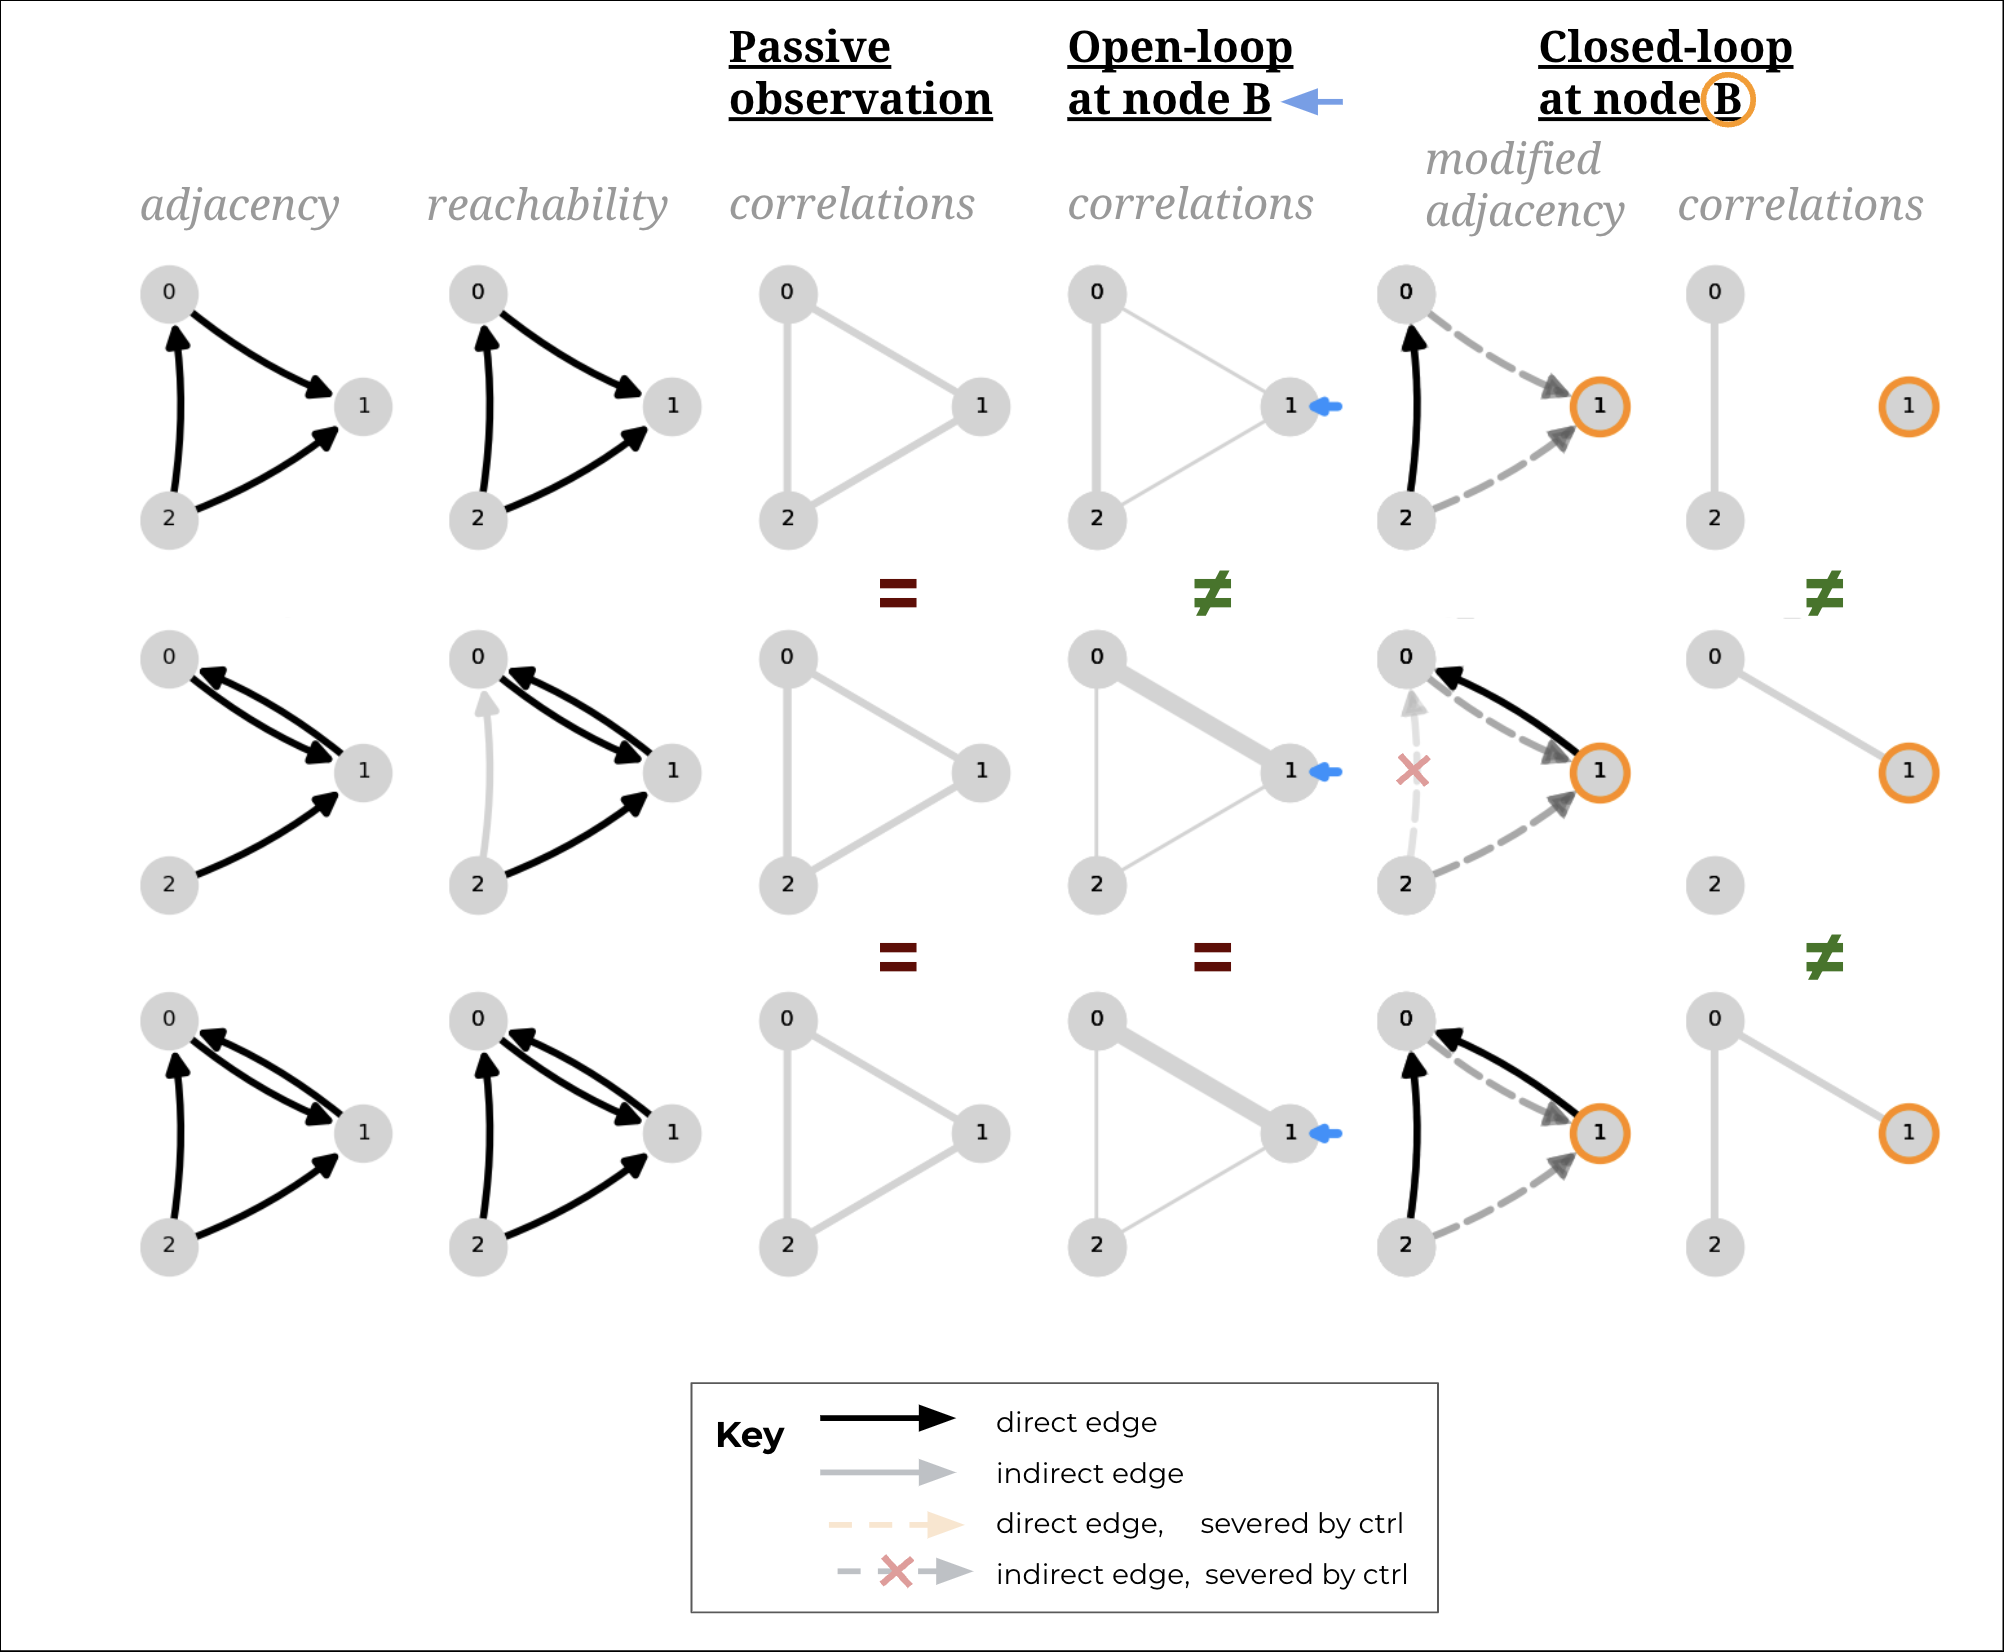
\includegraphics{figures/core_figure_sketches/circuit_walkthrough_3circuits_key_sketch.png}
\textgreater{} \textbf{Figure DEMO \emph{(box format)}: Applying CLINC
to distinguish a pair of circuits} \textgreater{} \textgreater{}
Consider the three-node identification problem shown in the figure
above, in which the experimenter has identified three hypotheses for the
causal structure of the circuit. These circuit hypotheses, shown as
directed graphs in column 1, can each also be represented by an
adjacency matrix of the form : for example, circuit A is represented by
an adjacency matrix in which \(w_{01}\), \(w_{20}\), and
\(w_{21} \neq 0\). Note that hypotheses A and C have direct connections
between nodes 0 and 2; while hypothesis B does not have a direct
connection between these nodes, computing the weighted reachability
matrix \(\widetilde{W}\) in circuit B an \emph{indirect} connection
exists through the path 2 \(\to\) 1 \(\to\) 0 (illustrated in gray in
column 2). \textgreater{} \textgreater{} Because there are direct or
indirect connections between each pair of nodes, passive observation of
each hypothesized circuit would reveal that each pair of nodes is
correlated (column 3). These three hypotheses are therefore difficult to
distinguish\footnote{saying ``difficult to distinguish'' instead of
  ``indistinguishable'' here since the magnitudes of the correlations
  could also be informative with different assumptions} for an
experimentalist who performs only passive observation, but can be
distinguished through stimulation. \textgreater{} \textgreater{} Column
4 shows the impact on observed correlations of performing
\emph{open-loop} control on node 1. In hypothesis A, node 1 is not a
driver of other nodes, so open-loop stimulation at this site will not
increase the correlation between the signal observed at node 1 and other
nodes. The path from node 1 to 0 in hypotheses B and C, meanwhile,
causes the open-loop stimulation at node 1 to \emph{increase} the
observed correlation between nodes 1 and 0. An experimenter can thus
distinguish between hypothesis A and the other two hypotheses by appling
open-loop control and observing the resulting pattern of correlations
(column 4). However, this pattern of open-loop stimulation would not
allow the experimenter to distinguish between hypotheses B and C.
\textgreater{} \textgreater{} \emph{Closed-loop} control (columns 5 and
6) can provide the experimenter with even more inferential power. Column
5 shows the resulting adjacency matrix when this closed-loop control is
applied to node 1. In each hypothesis, the impact of this closed-loop
control is to remove the impact of other nodes on node 1, because when
perfect closed-loop is applied the activity of node 1 is completely
independent of other nodes. (These severed connections are depicted in
column 5 by dashed lines.) In hypothesis B, this also results in the
elimation of the indirect connection from node 2 to node 1. The
application of closed-loop control at node 1 thus results in a different
observed correlation structure in each of the three circuit hypotheses
(column 6). This means that the experimenter can therefore distinguish
between these circuit hypotheses by applying closed-loop control -- a
task not possible with passive observation or open-loop control.

\hypertarget{theory-prediction}{%
\section{Theory / Prediction}\label{theory-prediction}}

FIG: %\includegraphics{figures/core_figure_sketches/methods_overview_pipeline_sketch.png}
\textgreater{} \textbf{Figure OVERVIEW:} \ldots{}

\hypertarget{predicting-correlation-structure-theory}{%
\subsection{Predicting correlation structure
(theory)}\label{predicting-correlation-structure-theory}}

A linear-Gaussian circuit can be described by 1) the variance of the
gaussian private (independent) noise at each node, and 2) the weight of
the linear relationships between each pair of connected nodes. Let
\(s \in \mathbb{R}^p\) denote the variance of each of the \(p\) nodes in
the circuit, and \(W \in \mathbb{R}^{p \times p}\) denote the matrix of
connection strengths such that
\[W_{ij} = \text{strength of $i \to j$ connection}.\]

Note that \(\left[(W^T) s\right]_j\) gives the variance at node \(j\)
due to length-1 (direct) connections, and more generally,
\(\left[ (W^T)^k s \right]_j\) gives the variance at node \(j\) due to
length-\(k\) (indirect) connections. The \emph{total} variance at node
\(j\) is thus \(\left[ \sum_{k=0}^{\infty} (W^T)^k s \right]_j\).

Our goal is to connect private variances and connection strengths to
observed pairwise correlations in the circuit. Defining
\(X \in \mathbb{R}^{p \times n}\) as the matrix of \(n\) observations of
each node, we have\footnote{To see this, denote by
  \(E \in \mathbb{R}^{p \times n}\) the matrix of \(n\) private noise
  observations for each node. Note that \(X = W^T X + E\), so
  \(X = E(I-W^T)^{-1}\). The covariance matrix
  \(\Sigma = \mathrm{cov}(X) = \mathbb{E}\left[X X^T\right]\) can then
  be written as
  \(\Sigma = \mathbb{E}\left[ (I-W^T)^{-1} E E^T (I-W^T)^{-1} \right] = (I-W^T)^{-1} \mathrm{cov}(E) (I-W^T)^{-T} = (I-W^T)^{-1} \mathrm{diag}(s) (I-W^T)^{-T}\).}
\[
\begin{aligned}
    \Sigma &= \mathrm{cov}(X) = \mathbb{E}\left[X X^T\right] \\
    &= (I-W^T)^{-1} \mathrm{diag}(s) (I-W^T)^{-T} \\
    &= \widetilde{W} \mathrm{diag}(s) \widetilde{W}^T,
\end{aligned}
\] where \(\widetilde{W} = \sum_{k=0}^{\infty} (W)^k\) denotes the
\emph{weighted reachability matrix}, whose \((i,j)^\mathrm{th}\) entry
indicates the total influence of node \(i\) on node \(j\) through both
direct and indirect connections.\footnote{We can use \(p-1\) as an upper
  limit on the sum \(\widetilde{W} = \sum_{k=0}^{\infty} W^k\) when
  there are no recurrent connections.} That is, \(\widetilde{W}_{ij}\)
tells us how much variance at node \(j\) would result from injecting a
unit of private variance at node \(i\). We can equivalently write
\(\Sigma_{ij} = \sum_{k=1}^p \widetilde{W}_{ik} \widetilde{W}_{jk} s_k\).

Under passive observation, the squared correlation coefficient can thus
be written as \[
\begin{aligned}
    r^2(i,j) &= \frac{\Sigma_{ij}}{\Sigma_{ii} \Sigma_{jj}} \\
    &= \frac{\left( \sum_{k=1}^p \widetilde{W}_{ik} \widetilde{W}_{jk} s_k \right)^2}{\left(\sum_{k=1}^p \widetilde{W}_{ik}^2 s_k\right)\left(\sum_{k=1}^p \widetilde{W}_{jk}^2 s_k\right)}.
\end{aligned}
\]

This framework also allows us to predict the impact of open- and
closed-loop control on the pairwise correlations we expect to observe.
To model the application of open-loop control on node \(c\), we add an
arbitrary amount of private variance to \(s_c\):
\(s_c \leftarrow s_c + s_c^{(OL)}\). To model the application of
closed-loop control on node \(c\), we first sever inputs to node \(c\)
by setting \(W_{k,c} = 0\) for \(k = 1, \dots p\), and then set the
private variance of node \(c\) by setting \(s_c\) to any arbitrary
value. Because \(c\)'s inputs have been severed, this private noise will
become exactly node \(c\)'s output variance.

\hypertarget{simulation-methods}{%
\section{Simulation Methods}\label{simulation-methods}}

\hypertarget{modeling-network-structure-and-dynamics}{%
\subsection{Modeling network structure and
dynamics}\label{modeling-network-structure-and-dynamics}}

We sought to understand both general principles (abstracted across
particulars of network implementation) as well as some practical
considerations introduced by dealing with spikes and synapses.

\hypertarget{stochastic-network-dynamics}{%
\subsubsection{Stochastic network
dynamics}\label{stochastic-network-dynamics}}

The first approach is accomplished with a network of nodes with gaussian
noise sources, linear interactions, and linear dynamics. The second
approach is achieved with a network of nodes consisting of populations
of leaky integrate-and-fire (LIF) neurons. These differ from the simpler
case in their nonlinear-outputs, arising from inclusion of a spiking
threshold. Interactions between neurons happen through spiking synapses,
meaning information is passed between neurons sparsely in
time\footnote{However, depending on overall firing rates and population
  sizes, this sparse spike-based transmission can be coarse-grained to a
  firing-rate-based model.}.

\emph{Neuron dynamics:} \[
\frac{dV}{dt} = \frac{V_0 + I - V}{\tau_m} + \sigma_m \sqrt{\tau_m} \xi(t)
\]

\hypertarget{time-resolvable-interactions}{%
\subsubsection{Time-resolvable
interactions}\label{time-resolvable-interactions}}

Additionally we study two domains of interactions between populations;
contemporaneous and delay-resolvable connections. These domains
represent the relative timescales of measurement versus timescale of
synaptic delay. \footnote{cases doesnt work with pandoc yet, also want
  to talk about positive and negative lags here}

In the delay-resolvable domain, directionality of connections may be
inferred even under passive observations by looking at temporal
precedence - whether the past of one signal is more strongly correlated
with future lags of another signal \emph{(i.e.~cross-correlation)}. In
the contemporaneous domain, network influences act within the time of a
single sample\footnote{the effective \(\Delta_{sample}\) would be
  broadened in the presence of jitter in connection delay, measurement
  noise, or temporal smoothing applied post-hoc, leading} so this
temporal precedence clue is lost (although directionality can still be
inferred in the presence of intervention).

The following work is presented with the linear-Gaussian and
contemporaneous domains as the default for simplicity and conciseness.

\hypertarget{code-implementation}{%
\subsubsection{Code implementation}\label{code-implementation}}

Software for data generation, analysis, and plotting is available at
https://github.com/awillats/clinc. Both linear-gaussian and spiking
networks are simulated with code built from the
\href{https://elifesciences.org/articles/47314}{Brian2} spiking neural
network simulator. This allows for highly modular code with easily
interchanged neuron models and standardized output preprocessing and
plotting. It was necessary to write an additional custom extension to
Brian2 in order to capture delayed linear-gaussian interactions,
available at
\href{https://github.com/awillats/brian_delayed_gaussian}{brian\_delayed\_gaussian}.
With this added functionality, it is possible to compare the equivalent
network parameters only changing linear-gaussian versus spiking dynamics
and inspect differences solely due to spiking.

\emph{see \url{_network_parameters_table.md} for list of relevant
parameters}

\hypertarget{implementing-interventions}{%
\subsection{Implementing
interventions}\label{implementing-interventions}}

FIG: %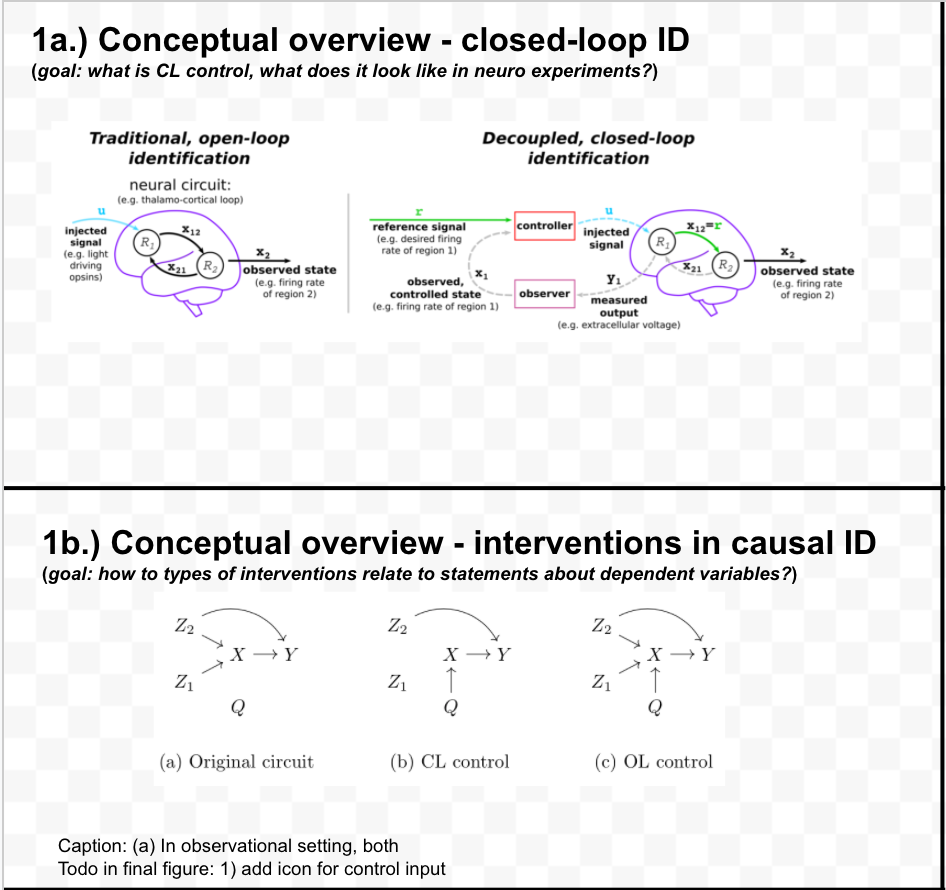
\includegraphics{figures/core_figure_sketches/figure1_sketch.png}

To study the effect of various interventions we simulated inputs to
nodes in a network. In the \textbf{passive setting}, nodes receive
additive drive from \emph{private} Gaussian noise sources common to all
neurons within a node, but independent across nodes. The variance of
this noise is specified by \(\sigma_m \sqrt{\tau_m}\).\footnote{need to
  triple check indexing w.r.t. nodes, neurons}

\[
\frac{dV}{dt} = \frac{V_0 + I - V}{\tau_m} + \sigma_m \sqrt{\tau_m} \xi(t)
\]

To emulate \textbf{open-loop intervention} we simulated current
injection from an external source. This is intended to represent
experiments involving stimulation from microelectrodes or optogenetics
\emph{(albeit simplifying away any impact of actuator dynamics)}. By
default, open-loop intervention is specified as white noise sampled at
each timestep from Gaussian distribution with mean and variance
\(\mu_{intv.}\) and \(\sigma^2_{intv.}\)\footnote{need to resolve
  differences in implementation between contemporaneous and voltage
  simulation cases}

\[ I_{open-loop} \sim \mathcal{N}(\mu_{intv.},\,\sigma^{2}_{intv.})\\
\] Ignoring the effect of signal means in the linear-Gaussian setting:
\[ X_k = f(\sigma^2_m, \sigma^{2}_{intv.})
\] \texttt{per-node\ indexing\ needs\ resolving\ here\ also}

Ideal \textbf{closed-loop control} is able to overwrite the output of a
node, setting it precisely to the specified target.
\texttt{making\ up\ notation\ as\ I\ go\ here,\ needs\ tightening\ up:}
\[
\begin{aligned} T &\sim \mathcal{N}(\mu_{intv.},\,\sigma^{2}_{intv.}) \\ I_{closed-loop} &= f(X, T)  \\ X_k | CL_{k} &\approx T
\end{aligned}
\] Note that in this setting, the \emph{output} of a node \(X_k\) under
closed-loop control is identical to the target, therefore
\[ X_k | CL_{k} = f(\sigma^{2}_{intv.}) \perp \sigma^2_m
\] In practice, near-ideal control is only possible with very fast
measurement and computation relative to the network's intrinsic
dynamics, such as in the case of dynamic clamp\footnote{NEED dynamic
  clamp refs - http://www.scholarpedia.org/article/Dynamic\_clamp}. To
demonstrate a broader class of closed-loop interventions (such as those
achievable with extracellular recording and stimulation), imperfect
``partial'' control is simulated by linearly interpolating the output of
each node between the target \(T\) and the uncontrolled output based on
a control effectiveness parameter \(\gamma\)

\[ X | CL_{k, \gamma} = \gamma T + (1-\gamma) X
\]

In the full discrete-time simulation, closed-loop interventions are
instead simulated through a proportional-integral-derivative (PID)
control policy with control efficacy determined functionally by the
strength of controller gains \(K = \{k_P, k_I, k_D\}\) relative to the
dynamics of the network.

\[I_{PID} = \text{PID}(X,T| K)\]

Another interesting intervention to study is \textbf{open-loop replay of
a closed-loop stimulus}, \emph{that is} taking a particular injected
current \(I_{CL,\,prev}\) used to drive nodes to a target \(T_{prev}\)
and adding it back to the network in a separate trial.

Because the instantiation of noise in the network will be different from
trial to trial, this ``replay'' stimulus will no longer adapt
sample-by-sample (therefore it should be considered open-loop) and the
node's output cannot be expected to match the target precisely, however
the statistics of externally applied inputs will be the same. In effect,
the comparison between closed-loop and open-loop replay conditions
reveals the specific effect of feedback intervention while controlling
for any confounds from input statistics.

\hypertarget{extracting-circuit-estimates}{%
\subsection{Extracting circuit
estimates}\label{extracting-circuit-estimates}}

While a broad range of techniques\footnote{\emph{inference techniques
  mentioned in the intro\ldots{}}} exist for inferring functional
relationships from observational data,
\texttt{(for\ the\ majority\ of\ this\ work)} we choose to focus on
simple bivariate correlation as a measure of dependence in the
linear-Gaussian network. The impact of intervention on this metric is
analytically tractable \emph{(see
\url{methods1_predicting_correlation.md})}, and can be thought of as a
prototype\footnote{what does ``prototype'' mean here? something like MI
  and corr are equivalent in the linear-Gaussian case, \ldots{}} for
more sophisticated measures of dependence such as time-lagged
cross-correlations, bivariate and multivariate transfer entropy.

We implement a naive comparison strategy to estimate the circuit
adjacency from emprical correlations; Thresholded empirical correlation
matrices are compared to correlation matrices predicted from each
circuit in a hypothesis set. Any hypothesized cirucits which are
predicted to have a similar correlation structure as is observed
(i.e.~corr. mats equal after thresholding) are marked as ``plausible
circuits.''\footnote{TODO? formalize notation for this} If only one
circuit amongst the hypothesis set is a plausible match, this is
considered to be the estimated circuit. The threshold for ``binarizing''
the empirical correlation matrix is treated as a hyperparameter to be
swept at the time of analysis.\footnote{not sure how important this is.
  would prefer to set this threshold at some ad-hoc value since we're
  sweeping other properties. But a more in-depth analysis could look at
  a receiver-operator curve with respect to this threshold}

\hypertarget{information-theoretic-measures-of-hypothesis-ambiguity}{%
\subsection{Information-theoretic measures of hypothesis
ambiguity}\label{information-theoretic-measures-of-hypothesis-ambiguity}}

\emph{see \url{_steps_of_inference.md} for entropy writeup}

\hypertarget{results}{%
\section{Results}\label{results}}

\hypertarget{impact-of-intervention-on-estimation-performance}{%
\subsection{Impact of intervention on estimation
performance}\label{impact-of-intervention-on-estimation-performance}}

\hypertarget{intervening-provides-categorical-improvements-in-inference-power-beyond-passive-observation}{%
\subsubsection{Intervening provides (categorical) improvements in
inference power beyond passive
observation}\label{intervening-provides-categorical-improvements-in-inference-power-beyond-passive-observation}}

Next, we apply (steps 1-3 of) this circuit search procedure to a
collection of closely related hypotheses for 3 interacting
nodes\footnote{nodes in such a graphical model may represent populations
  of neurons, distinct cell-types, different regions within the brain,
  or components of a latent variable represented in the brain.} to
illustrate the impact of intervention. ???
\texttt{most\ of\ the\ story\ in\ the\ figure\ caption\ for\ now} ???

FIG: %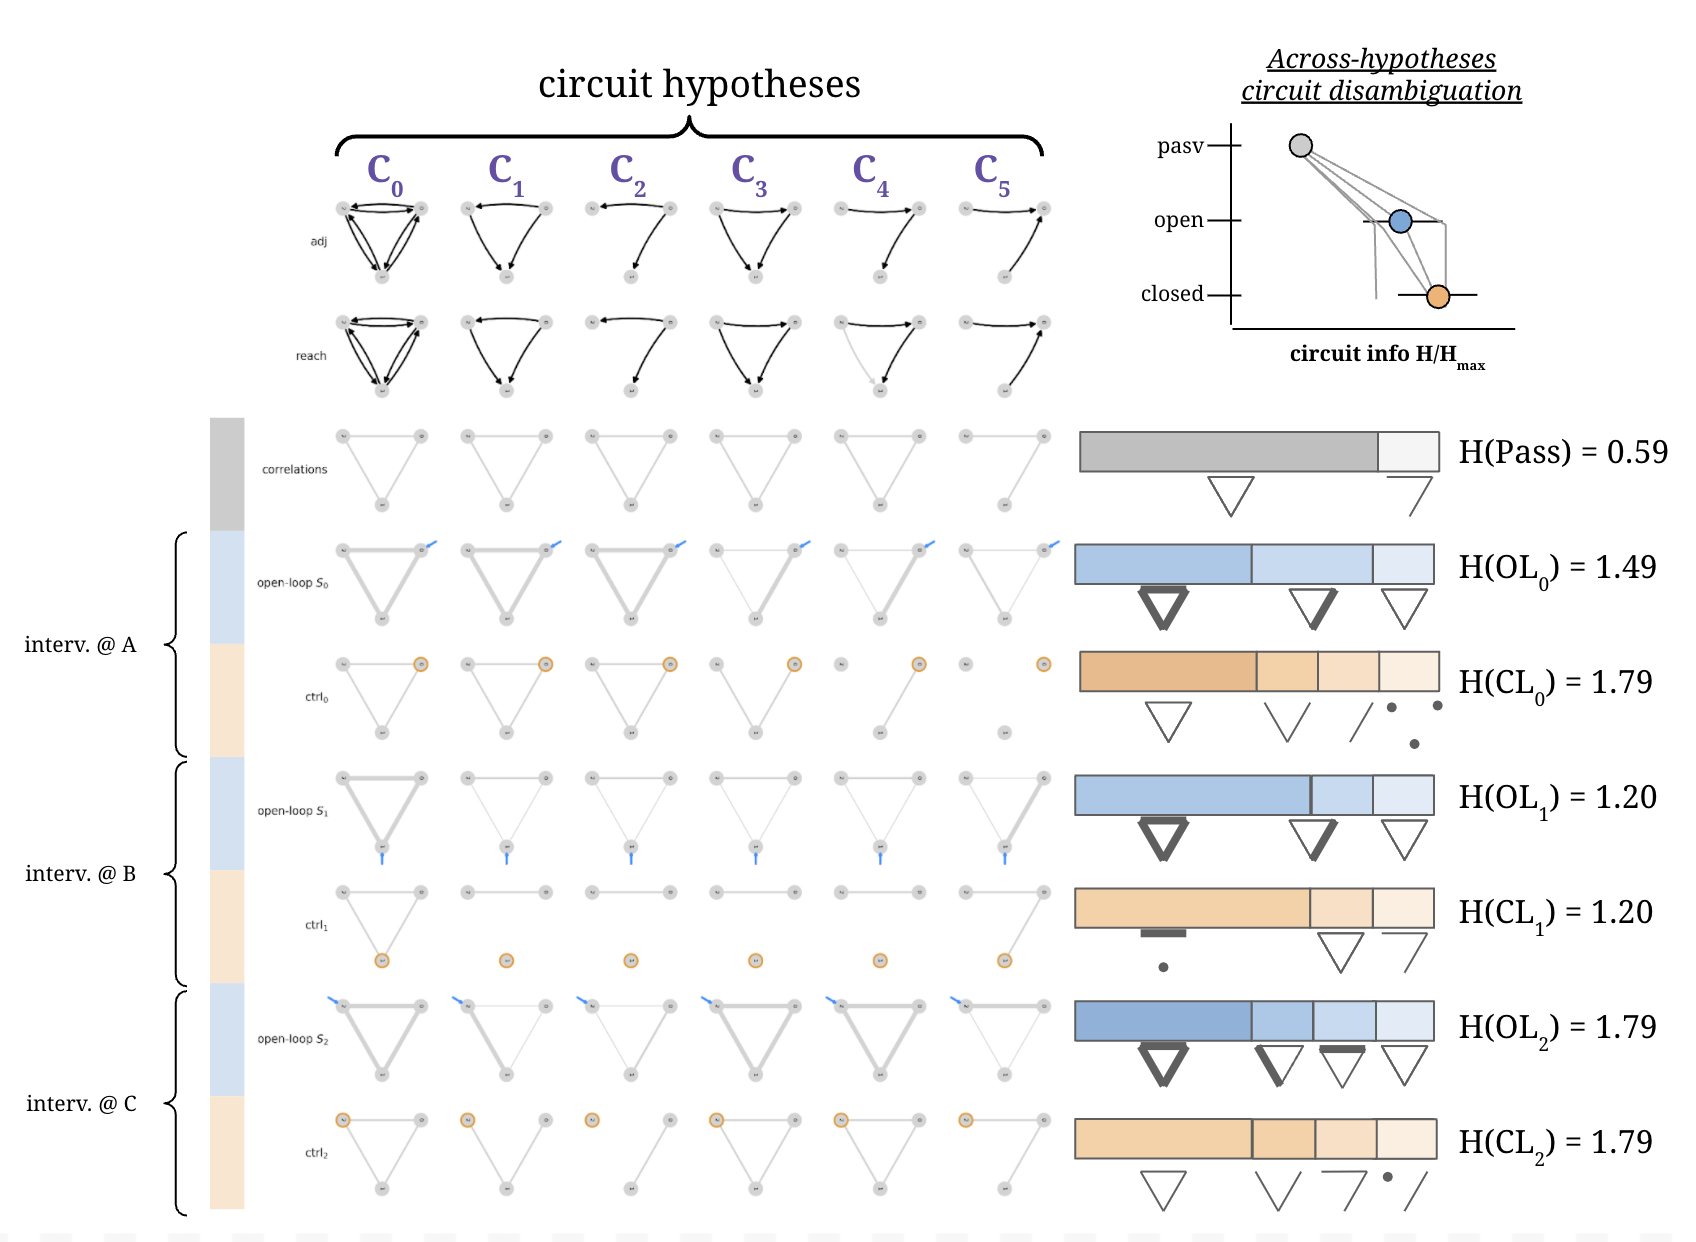
\includegraphics{figures/core_figure_sketches/circuit_entropy_sketch.png}
\textgreater{} \textbf{Figure DISAMBIG: Interventions narrow the set of
hypotheses consistent with observed correlations} \emph{source:
\href{https://docs.google.com/drawings/d/1CBp1MhOW7OGNuBvo7OkIuzqnq8kmN8EEX_AkFuKpVtM/edit}{google
drawing}} \textgreater{}\textbf{(A)} Directed adjacency matrices
represent the true and hypothesized causal circuit structure
\textgreater{}\textbf{(B)} Directed reachability matrices represent the
direct \emph{(black)} and indirect \emph{(grey)} influences in a
network. Notably, different adjacency matrices can have equivalent
reachability matrices making distinguishing between similar causal
structures difficult, even with open-loop control.
\textgreater{}\textbf{(C)} Correlations between pairs of nodes. Under
passive observation, the direction of influence is difficult to
ascertain. In densely connected networks, many distinct ground-truth
causal structures result in similar ``all correlated with all'' patterns
providing little information about the true structure.
\textgreater{}\textbf{(D-F)} The impact of open-loop intervention at
each of the nodes in the network is illustrated by modifications to the
passive correlation pattern. Thick orange\footnote{will change the color
  scheme for final figure. Likely using orange and blue to denote closed
  and open-loop interventions. Will also add in indication of severed
  edges} edges denote correlations which increase above their baseline
value with high variance open-loop input. Thin blue\footnote{will change
  the color scheme for final figure. Likely using orange and blue to
  denote closed and open-loop interventions. Will also add in indication
  of severed edges} edges denote correlations which decrease, often as a
result of increased connection-independent ``noise'' variance in one of
the participating nodes. Grey edges are unaffected by intervention at
that location. \textgreater{} A given hypotheses set (A) will result in
an ``intervention-specific fingerprint'', that is a distribution of
frequencies for observing patterns of modified correlations
\emph{(across a single row within D-F)}. If this fingerprint contains
many examples of the same pattern of correlation (such as \textbf{B}),
many hypotheses correspond to the same observation, and that experiment
contributes low information to distinguish between structures. A
maximally informative intervention would produce a unique pattern of
correlation for each member of the hypothesis set.
:construction:\texttt{caption\ too\ long}

\textbf{Why does closed-loop control provide a categorical advantage?}
Because it severs indirect links
\texttt{is\ this\ redundant\ with\ intro?}
\texttt{needs\ to\ be\ backed\ here\ up\ by\ aggregate\ results?} - this
is especially relevant in recurrently connected networks where the
reachability matrix becomes more dense. - more stuff is connected to
other stuff, so there are more indirect connections, and the resulting
correlations look more similar (more circuits in the equivalence class)
- patterns of correlation become more specific with increasing
intervention strength - more severed links \(\rightarrow \) more unique
adjacency-specific patterns of correlation

\begin{quote}
\textbf{Where you intervene}\footnote{Figure VAR shows this pretty well,
  perhaps sink this section until after discussing categorical and
  quantitative?} strongly determines the inference power of your
experiment. \textbf{secondary point:} having (binary) prediction helps
capture this relationship
\end{quote}

\hypertarget{stronger-intervention-shapes-correlation-resulting-in-more-data-efficient-inference-with-less-bias}{%
\subsubsection{Stronger intervention shapes correlation, resulting in
more data-efficient inference with less
bias}\label{stronger-intervention-shapes-correlation-resulting-in-more-data-efficient-inference-with-less-bias}}

While a primary advantage of closed-loop interventions for circuit
inference is its ability to functionally lesion indirect connections,
another, more nuanced \texttt{(quantitative)} advantage of closed-loop
control lies in its capacity to bidirectionally control output variance.
While the variance of an open-loop stimulus can be titrated to adjust
the output variance at a node, in general, an open-loop stimulus cannot
reduce this variance below its instrinsic\footnote{below the level set
  by added, independent/``private'' sources} variability. That is, if
the system is linear with gaussian noise,

\[\mathbb{V}_{i}(C|S=\text{open},\sigma^2_S) \geq \mathbb{V}_{i}(C)\]
More specifically, if the open-loop stimulus is statistically
independent from the intrinsic variability\footnote{notably, this is
  part of the definition of open-loop intervention}
\[\mathbb{V}_{i}(C|S=\text{open},\sigma^2_S) = \mathbb{V}_{i}(C) + \sigma^2_S\]
Applying closed-loop to a linear gaussian circuit:

\[
\begin{aligned}
\mathbb{V}_{i}(C|S=\text{closed},\sigma^2_S) &= \sigma^2_S  \\
\mathbb{V}_{i}(C|S=\text{closed},\sigma^2_S) &\perp \mathbb{V}_{i}(C)
\end{aligned}
\]

\hypertarget{impact-of-intervention-location-and-variance-on-pariwise-correlations}{%
\paragraph{Impact of intervention location and variance on pariwise
correlations}\label{impact-of-intervention-location-and-variance-on-pariwise-correlations}}

\href{methods1_predicting_correlation.md}{related methods}

We have shown that closed-loop interventions provide more flexible
control over output variance of nodes in a network, and that shared and
independent sources of variance determine pairwise correlations between
node outputs. Together, this suggests closed-loop interventions may
allow us to shape the pattern of correlations with more degrees of
freedom\footnote{need a more specific way of stating this. I mean
  degrees of freedom in the sense that mean and variance can be
  controlled independent of each other. And also, that the range of
  achievable correlation coefficients is wider for closed-loop than
  open-loop (where instrinsic variability constrains the minimum output
  variance)} \texttt{{[}why\ do\ we\ want\ to?...{]}}

One application of this increased flexibility is to increase
correlations associated with pairs of directly correlated nodes, while
decreasing spurious correlations associated with pairs of nodes without
a direct connection (but perhaps are influenced by a common input, or
are connected only indirectly). While ``correlation does not imply
causation,'' intervention may decrease the gap between the two.

Our hypothesis is that this shaping of pairwise correlations will result
in reduced false positive edges in inferred circuits, ``unblurring'' the
indirect associations that would otherwise confound circuit inference.
However care must be taken, as this strategy relies on a hypothesis for
the ground truth adjacency and may also result in a ``confirmation
bias'' as new spurious correlations can be introduced through
closed-loop intervention.

The impact of intervention on correlations can be summarized through the
co-reachability \(\text{CoReach}(i,j|S_k)\). A useful distillation of
this mapping is to understand the sign of \(\frac{dR_{ij}}{dS_k}\), that
is whether increasing the variance of an intervention at node \(k\)
increases or decreases the correlation between nodes \(i\) and \(j\)

In a simulated network \(A\rightarrow B\)
\protect\hyperlink{fig-var}{(fig.~variance)} we demonstrate predicted
and emprirical correlations between a pair of nodes as a function of
intervention type, location, and variance. A few features are present
which provide a general intuition for the impact of intervention
location in larger circuits: First, interventions ``upstream'' of a true
connection \protect\hyperlink{fig-var}{(lower left, fig.~variance)} tend
to increase the connection-related variance, and therefore strengthen
the observed correlations.
\[\text{Reach}(S_k\rightarrow i) \neq 0 \\ \text{Reach}(i\rightarrow j) \neq 0 \\ \frac{dR}{dS_k} > 0\]

Second, interventions affecting only the downstream node
\protect\hyperlink{fig-var}{(lower right, fig.~variance)} of a true
connection introduce variance which is independent of the connection
\(A\rightarrow B\), decreasing the observed correlation.
\[\text{Reach}(S_k \rightarrow  j) = 0 \\ \text{Reach}(S_k \rightarrow  j) \neq 0 \\ \frac{dR}{dS_k} < 0\]

Third, interventions which reach both nodes will tend to increase the
observed correlations \protect\hyperlink{fig-var}{(upper left,
fig.~variance)}, moreover this can be achieved even if no direct
connection \(i\rightarrow j\) exists.
\[\text{Reach}(S_k \rightarrow  i) \neq 0 \\ \text{Reach}(S_k \rightarrow  j) \neq 0 \\ \text{Reach}(i \rightarrow  j) = 0 \\ \frac{dR}{dS_k} > 0\]

Notably, the impact of an intervention which is a ``common cause'' for
both nodes depends on the relative weighted reachability between the
source and each of the nodes. Correlations induced by a common cause are
maximized when the input to each node is equal, that is
\(\widetilde{W}_{S_k\rightarrow i} \approx \widetilde{W}_{S_k\rightarrow j}\) (upper right *
in \protect\hyperlink{fig-var}{fig.~variance}). If \(i\rightarrow j\) are connected
\(\widetilde{W}_{S_k\rightarrow i} \gg \widetilde{W}_{S_k\rightarrow j}\) results in an
variance-correlation relationship similar to the ``upstream source''
case (increasing source variance increases correlation
\(\frac{dR}{dS_k} > 0\)), while
\(\widetilde{W}_{S_k\rightarrow i} \ll \widetilde{W}_{S_k\rightarrow j}\) results in a
relationship similar to the ``downstream source'' case
(\(\frac{dR}{dS_k} < 0\))\footnote{not 100\% sure this is true, the
  empirical results are really pointing to dR/dW\textless0 rather than
  dR/dS\textless0. Also this should really be something like
  \(\frac{d|R|}{dS}\) or \(\frac{dr^2}{dS}\) since these effects
  decrease the \emph{magnitude} of correlations. I.e. if
  \(\frac{d|R|}{dS} < 0\) increasing \(S\) might move \(r\) from
  \(-0.8\) to \(-0.2\), i.e.~decrease its magnitude not its value.}

FIG: %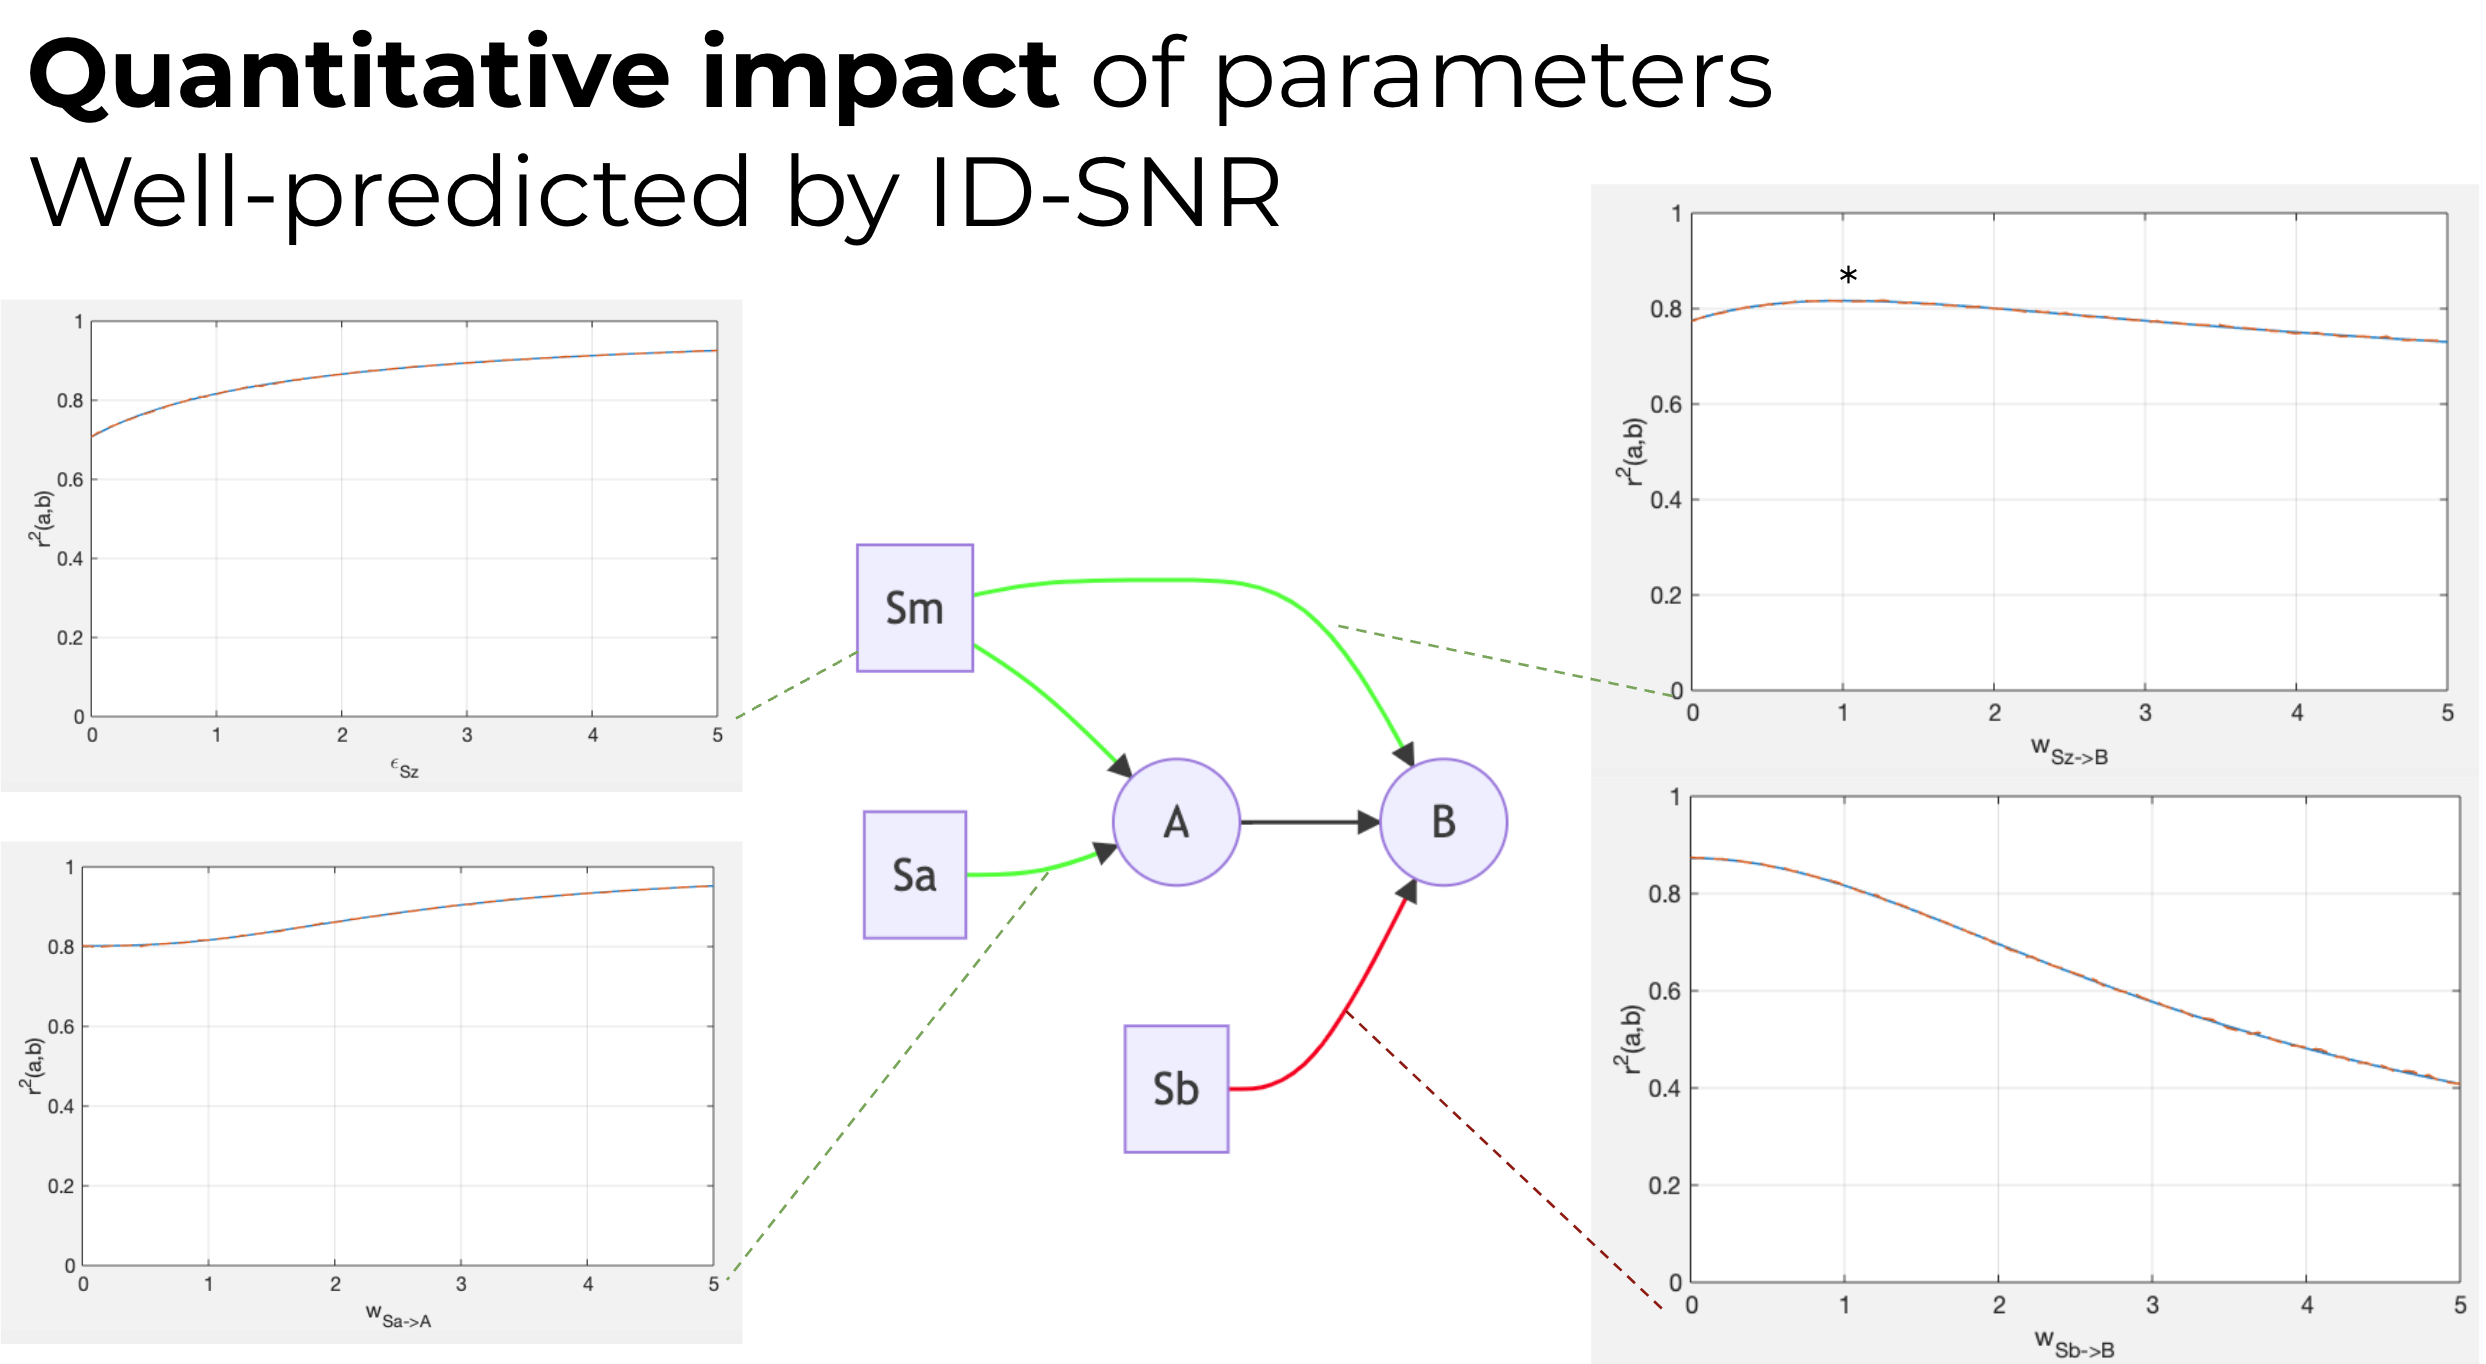
\includegraphics{figures/misc_figure_sketches/quant_r2_prediction_common.png}
FIG: %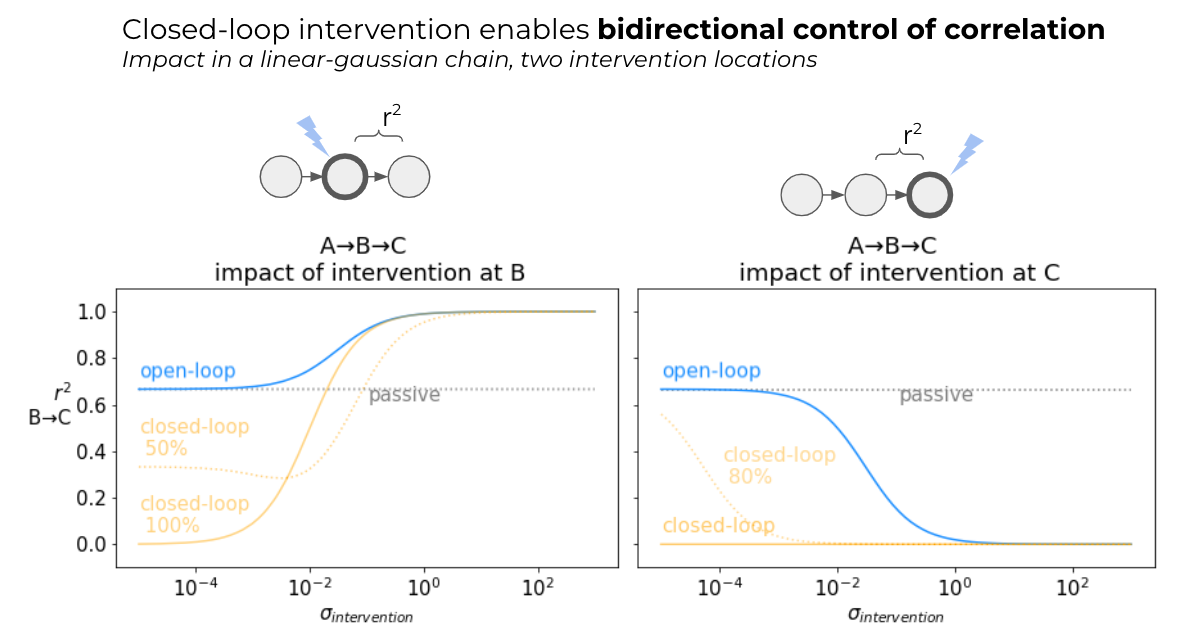
\includegraphics{figures/from_code/bidirectional_correlation.png}

\begin{quote}
???(Final figure will be a mix of these two panels, caption will need
updating) \textbf{Figure VAR: Location, variance, and type of
intervention shape pairwise correlations} \textbf{(CENTER)} A two-node
linear gaussian network is simulated with a connection from \(A\rightarrow B\).
Open-loop interventions \emph{(blue)} consist of independent gaussian
inputs with a range of variances \(\sigma^2_S\). Closed-loop
interventions \emph{(orange)} consist of feedback control with an
independent gaussian target with a range of variances. \emph{Incomplete
closed-loop interventions result in node outputs which are a mix of the
control target and network-driven activity}. Connections from sources to
nodes are colored by their impact on correlations between A and B; green
denotes \(dR/dS > 0\), red denotes \(dR/dS<0\). \textbf{(lower left)}
Intervention ``upstream'' of the connection \(A\rightarrow B\) increases the
correlation \(r^2(A,B)\). \textbf{(lower right)} Intervention at the
terminal of the connection \(A\rightarrow B\) decreases the correlation
\(r^2(A,B)\) by adding connection-independent noise. \textbf{(upper
left)} Intervention with shared inputs to both nodes generally increases
\(r^2(A,B)\), \emph{(even without \(A\rightarrow B\), see supplement)}.
\textbf{(upper right)} The impact of shared interventions depends on
relative weighted reachability
\(\text{Reach}(S_k\rightarrow A) / \text{Reach}(S_k\rightarrow B)\), with highest correlations
when these terms are matched (see \emph{) Closed-loop interventions
}(orange)* generally result in larger changes in correlation across
\(\sigma^2_S\) than the equivalent open-loop intervention. Closed-loop
control at B effectively lesions the connection \(A\rightarrow B\), resulting in
near-zero correlation. \footnote{compare especially to
  \href{https://www.frontiersin.org/articles/10.3389/fncom.2020.00045/full}{``Transfer
  Entropy as a Measure of Brain Connectivity''},
  \href{https://www.jneurosci.org/content/29/33/10234}{``How
  Connectivity, Background Activity, and Synaptic Properties Shape the
  Cross-Correlation between Spike Trains''} Figure 3.}
\end{quote}

??? The change in correlation as a function of changing intervention
variance (\(\frac{dr^2_{ij}}{dS}\)) can therefore be used as an
additional indicator of presence/absence and directionality of the
connection between A,B \emph{(see \href{fig-disambig}{fig.~disambig.
D.)})} ???

\protect\hyperlink{fig-var}{Fig. variance} also demonstrates the
relative dynamic range of correlations achievable under passive, open-
and closed-loop intervention. In the passive case, correlations are
determined by instrinsic properties of the network \(\sigma^2_{base}\).
These properties have influence over the observed correlations in a way
that can be difficult to separate from differences due to the
ground-truth circuit. With open-loop intervention we can observe the
impact of increasing variance at a particular node, but the dynamic
range of achievable correlations is bounded by not being able to reduce
variance below its baseline level. With closed-loop control, the
bidirectional control of the output variance for a node means a much
wider range of correlations can be achieved
\protect\hyperlink{fig-var}{(blue v.s. orange in fig.~variance)},
resulting in a more sensitive signal reflecting the ground-truth
connectivity.

\emph{see also \url{results1B_data_efficiency_and_bias.md}}

\hypertarget{discussion}{%
\section{Discussion}\label{discussion}}

\hypertarget{limitations}{%
\subsubsection{limitations}\label{limitations}}

The examples explored in this work simplify several key features that
may have relevant contributions to circuit identification in practical
experiments. {[}\ldots{]}

\texttt{full\ observability}

\hypertarget{results-summary-to-summary-of-value-closed-loop-generally}{%
\subsubsection{results summary to summary of value closed-loop
generally}\label{results-summary-to-summary-of-value-closed-loop-generally}}

Closed-loop control has the disadvantages of being more complex to
implement and requires specialized real-time hardware and software,
however it has been shown to have multifaceted usefulness in clinical
and basic science applications. Here we focused on two advantages in
particular; First, the capacity for functional lesioning which
(reversibly) severs inputs to nodes and second, closed-loop control's
capacity to precisely shape variance across nodes. Both of these
advantages facilitate opportunities for closed-loop intervention to
reveal more circuit structure than passive observation or even open-loop
experiments.

\hypertarget{summary-of-guidelines-for-experimentors}{%
\subsubsection{summary of guidelines for
experimentors}\label{summary-of-guidelines-for-experimentors}}

In studying the utility of various intervention for circuit inference we
arrived at a few general guidelines which may assist experimental
neuroscientists in designing the right intervention for the quesiton at
hand. First, more ambiguous hypotheses sets require ``stronger''
interventions to distinguish. Open-loop intervention may be sufficient
to determine directionality of functional relationships, but as larger
numbers of similar hypotheses {[}\ldots{]} closed-loop intervention
reduces the hypothesis set more efficiently. Second, we find that dense
networks with strong reciprocal connections tend to result in many
equivalent circuit hypotheses, but that well-placed closed-loop control
can disrupt loops and simplify correlation structure to be more
identifiable.\footnote{this corroborates Ila Fiete's paper on bias as a
  function of recurrent network strength} Recurrent loops are a common
feature of neural circuit, and represent key opportunities for
successful closed-loop intervention. The same is true for circuits with
strong indirect correlations

\texttt{hidden\ confounds}

\hypertarget{funnel-out-future-work-to-broad-impact}{%
\subsubsection{``funnel out'', future work to broad
impact}\label{funnel-out-future-work-to-broad-impact}}

\texttt{sequential\ experimental\ design}

\emph{see
\href{/sketches_and_notation/discussion/limitations_future_work.md}{limitations\_future\_work.md}}

\hypertarget{references}{%
\section{References}\label{references}}

\emph{see
\href{https://github.com/shd101wyy/markdown-preview-enhanced/blob/master/docs/pandoc-bibliographies-and-citations.md}{pandoc
pandoc-citations}}
